% -*- coding:utf-8 -*-
% AutoFakeBold和AutoFakeSlant是xeCJK宏包中的选项,开启伪粗体和伪斜体
% 行距被设定为linespread=1.65,这是最接近word中1.5倍行距的效果
\documentclass[a4paper,UTF8,twoside,zihao=-4,no-math,linespread=1.65,AutoFakeBold=1.8,AutoFakeSlant=true]{ctexrep}
\normalsize	                  % 字号(因为在文档类选项里面指定了zihao=-4,所以默认小4号字)
\setlength{\parskip}{0ex}     % 段落间的间距

%---------加载宏包----------
\usepackage{fontspec}	      % 设置英文字体
\setmainfont{Times New Roman}
\usepackage{amsmath}	      % 数学公式
\usepackage{amssymb}	      % 数学符号
\usepackage{amsthm}		      % 数学定理
\usepackage[top=3.3cm,bottom=3.3cm,left=3.17cm,right=3.17cm,headsep=0.7cm,headheight=0.5cm,footskip=1.25cm]{geometry} % 页边距
\usepackage{float}            % 调整浮动体可用“[H]”固定图表插入位置
\usepackage{hvfloat}          % 调整浮动体可用于横置图表
\usepackage{graphicx}	      % 插入图片
\usepackage{adjustbox}        % 调整box环境
\usepackage{tabu}             % 跨页长表格
\usepackage{longtable}        % 跨页长表格
\usepackage{booktabs}	      % 三线表
\usepackage{multirow}	      % 合并行单元格
\usepackage{hyperref}	      % 链接宏包
\hypersetup{hidelinks}        % 隐藏链接
\usepackage[backend=biber,style=gb7714-2015,gbpub=false,gbalign=gb7714-2015]{biblatex} % 参考文献格式gb7714-2015
%--------------修改对齐环境以使参考文献不悬挂缩进--------------
\setlength{\biblabelsep}{2mm} % 顺序标签与文献内容的间距
\renewcommand{\itemcmd}{%
\addvspace{\bibitemsep}       % 恢复\bibitemsep的作用
\mkgbnumlabel{\printfield{labelnumber}}%
\hspace{\biblabelsep}}
%------------------------------------------------------------
\addbibresource{ref.bib}      % biblatex参考文献库

%--------------------设置目录格式和引导点--------------------- 
\usepackage{tocloft} 
\renewcommand{\cftdotsep}{1}                  % 设置引导点间隔
\setlength{\cftbeforetoctitleskip}{0pt}       % 目录标题前的空白设为0
\setlength{\cftaftertoctitleskip}{0pt}        % 目录标题后的空白设为0
\renewcommand{\contentsname}{目 \quad 录}
\renewcommand{\cftchapleader}{\cftdotfill{\cftdotsep}}
\renewcommand\cfttoctitlefont{\heiti\zihao{-3}}
\renewcommand\cftchapfont{\normalsize}
\renewcommand\cftsecfont{\normalsize}
\renewcommand\cftsubsecfont{\normalsize}
\renewcommand\cftchappagefont{\normalsize}
\renewcommand\cftsecpagefont{\normalsize}
\renewcommand\cftsubsecpagefont{\normalsize}

\usepackage[style=base,justification=centering,font=small]{caption}	% 更改标题要用到的宏包
\DeclareCaptionLabelSeparator{nocolon}{~}							% 图编号与标题之间不带冒号
\captionsetup{labelsep=nocolon}										% 图编号与标题之间不带冒号
\renewcommand{\thefigure}{\thechapter-\arabic{figure}}				% 设置图标题的连接符是-
\renewcommand{\thetable}{\thechapter-\arabic{table}}				% 设置表标题的连接符是-
\renewcommand{\theequation}{\thechapter-\arabic{equation}}			% 设置公式编号的连接符是-
\renewcommand{\footnotesize}{\small\selectfont}                     % 设置脚注字号为五号

\usepackage{fancyhdr}        % 设置页眉页脚
\fancypagestyle{plain}{%
\fancyhf{}                   % 清空页眉页脚 
\fancyfoot[C]{\thepage}      % 页脚为页码
\cfoot{\zihao{-5}{\thepage}} % 页码字号小五
\renewcommand{\headrulewidth}{0pt}
\renewcommand{\footrulewidth}{0pt}}

%---------设置各种间距-----------
\setlength{\intextsep} {3.5ex plus 0.2ex minus 0.2ex}			    % 浮动体与文字之间的距离
\setlength{\textfloatsep} {3.5ex plus 0.2ex minus 0.2ex}		    % 浮动体与页面顶部或者底部的距离
\setlength{\floatsep} {3ex}										    % 两个浮动体之间的距离
\setlength{\abovecaptionskip} {1ex plus 0.2ex minus 0.2ex }		    % 浮动体与标题之间的距离
\setlength{\belowcaptionskip} {-1.0ex plus 0.2ex minus 0.2ex}

%---------设置章节标题格式----------
\ctexset{chapter={
	number=\arabic{chapter},
	format=\heiti\zihao{2}\centering,			% 2号黑体
	beforeskip=3ex plus 0.3ex minus 0.3ex,		% 与正文内容的间距
	afterskip=3ex plus 0.3ex minus 0.3ex,
	fixskip=true,
	name={}
	},
  section={
	format=\heiti\zihao{3},			            % 3号黑体
	beforeskip=1ex plus 0.1ex minus 0.1ex,		% 与正文内容的间距
	afterskip=1ex plus 0.1ex minus 0.1ex,
	},
  subsection={
	format=\heiti\zihao{4},						% 4号黑体
	beforeskip=1ex plus 0.1ex minus 0.1ex,	    % 与正文内容的间距
	afterskip=1ex plus 0.1ex minus 0.1ex,
	},
}

%--------图的路径和大小---------
\newcommand{\figpath}{../图}
\newcommand{\figwidth}{13cm}
\graphicspath{{figures/}}                       % 定义所有的图片文件在figures子目录下

%----------文档信息-------------
\newcommand\timu{论玄铁剑法在实战中的应用}
\newcommand\zuozhe{杨过}
\newcommand\xuehao{\textbf{1234567890}}
\newcommand\daoshi{郭靖}
\newcommand\daoshizhicheng{教授}
\newcommand\zhuanye{武术研究}
\newcommand\fangxiang{黯然销魂掌}
\newcommand\riqi{1250年5月}

\newcommand\yingwentimu{On the Application of Genteel Sword Technique in Practical Combat}
\newcommand\yingwenzuozhe{Guo Yang}
\newcommand\yingwenzhuanye{Martial Arts}
\newcommand\yingwenfangxiang{An Ran Xiao Hun Zhang}
\newcommand\yingwendaoshi{Jing Guo}
\newcommand\yingwenzhicheng{Prof.}

%----------开始正文----------------
\begin{document}
\songti			                 % 设定字体
\abovedisplayskip 2ex			 % 设置公式与正文的间隔
\belowdisplayskip 2ex
\abovedisplayshortskip 2ex
\belowdisplayshortskip 2ex

\begin{titlepage}
% -*- coding:utf-8 -*-

{
\cleardoublepage
\thispagestyle{empty}
\setlength{\parindent}{0em}
\songti\fontsize{15pt}{0pt}\selectfont 分类号 \hfill 密级 \phantom{密级}
\begin{center}
\vskip 30pt
\fangsong\fontsize{26pt}{0pt}\selectfont 中国地质大学(北京)
\vskip 35pt
\fangsong\fontsize{42pt}{0pt}\selectfont  \textbf{硕\ \ 士\ \ 学\ \ 位\ \ 论\ \ 文}
\vskip 80pt
\heiti\fontsize{26pt}{25pt}\selectfont {\timu}
\vskip 80pt

\fangsong\fontsize{16pt}{20pt}\selectfont
\begin{tabular}{p{34mm} p{55mm}}
  \textbf{学\hspace{\stretch{1}}号}&: \xuehao  \\
  \textbf{研\hspace{\stretch{1}}究\hspace{\stretch{1}}生}&: \textbf{\zuozhe}  \\
  \textbf{专\hspace{\stretch{1}}业}&: \textbf{\zhuanye}  \\
  \textbf{研\hspace{\stretch{1}}究\hspace{\stretch{1}}方\hspace{\stretch{1}}向}&: \textbf{\fangxiang}  \\
  \textbf{指\hspace{\stretch{1}}导\hspace{\stretch{1}}教\hspace{\stretch{1}}师}&: \textbf{\daoshi} ~ \textbf{\daoshizhicheng}
\end{tabular}

\vskip 60pt
\songti\fontsize{16pt}{0pt}\selectfont \riqi
\end{center}

\clearpage
\thispagestyle{empty}
%\ 
%\vskip 20pt
\fontsize{16pt}{22pt}\selectfont\centering \textbf{A Dissertation Submitted to}

\textbf{China University of Geosciences for Master Degree}
\vskip 120pt
\textbf{\yingwentimu}
\vskip 130pt
\raggedright
\setlength{\leftskip}{40pt}
\textbf{Master Candidate : \yingwenzuozhe}  \\
\textbf{Major : \yingwenzhuanye}  \\
\textbf{Study Orientation : \yingwenfangxiang}\\
\textbf{Dissertation Supervisor : \yingwenzhicheng ~ \yingwendaoshi}\\
\vskip 50pt
\centering \textbf{China University of Geosciences (Beijing)}

}
		 % 封面(盲审时可用title_anonymous)
% -*- coding:utf-8 -*-

{
\clearpage
\thispagestyle{empty}
%\ 
%\vskip 10pt
\heiti \LARGE \centering 声~明
\vskip 15pt
\songti \normalsize \raggedright \hspace{2em}本人声明所呈交的论文是我个人在导师指导下进行的研究工作及取得的研究成果。尽我所知,除了文中特别加以标注和致谢的地方外,论文中不包含其他人已经发表或撰写过的研究成果,也不包含为获得中国地质大学(北京)或其它教育机构的学位或证书而使用过的材料。与我一同工作的同志对本研究所做的任何贡献均已在论文中作了明确的说明并表示了谢意。

\vskip 60pt
\raggedleft \fontsize{13pt}{0pt}\selectfont 签~名:\underline{\hspace{3cm}}日~期: \underline{\hspace{3cm}}

\vskip 100pt
\centering \heiti \LARGE 关于论文使用授权的说明
\vskip 10pt

\songti \normalsize \raggedright \hspace{2em}本人完全了解中国地质大学(北京)有关保留、使用学位论文的规定,即:学校有权保留送交论文的复印件,允许论文被查阅和借阅;学校可以公布论文的全部或部分内容,可以采用影印、缩印或其他复制手段保存论文。
\vskip 20pt

\hspace{2em}$\square$公开\hspace{0.5cm}$\square$保密(\underline{\hspace{1cm}}年)\hspace{1cm}\fontsize{13pt}{0pt}\selectfont \textbf{(保密的论文在解密后应遵守此规定)}

\vskip 60pt
\songti \fontsize{13pt}{0pt}\selectfont 签~名:\underline{\hspace{3cm}}导师签名:\underline{\hspace{3cm}}日~ 期:\underline{\hspace{3cm}}	    	
}	 % 保密声明
\end{titlepage}

\pagenumbering{arabic}			 % 开始页码,格式为阿拉伯数字
\pagestyle{plain}				 % 不要页眉
% -*- coding:utf-8 -*-

{
\ctexset{chapter={
        format=\heiti\zihao{-3}\centering,	% 3号黑体
        %beforeskip=0ex,					% 与正文内容的间距
        %afterskip=1ex,
        numbering=false
    },
}
\chapter{摘要}
\zhlipsum[1-2]

\noindent \textbf{关键词:}关键词1,关键词2,关键词3,关键词4

\clearpage
}
 % 中文摘要
% -*- coding:utf-8 -*-

{
% 摘要用section实现,所以需要临时修改一下section的标题格式
\ctexset{chapter={
        format=\heiti\zihao{-3}\bfseries\centering,	% 3号黑体
        %beforeskip=0ex,							% 与正文内容的间距
        %afterskip=1ex,
        numbering=false
    },
}
\chapter{Abstract}
\lipsum[1-2]

\noindent \textbf{Key words:} keyword1, keyword2, keyword2, keyword3, Keyword4
}
	 % 英文摘要
\clearpage

\begin{center}
	\tableofcontents             % 生成目录
\end{center}

\clearpage
%-----------------------设置页眉页脚-------------------------------					        
\fancyhf{}\renewcommand*{\headrulewidth}{0.75bp}
\fancyhead[L]{}
\fancyhead[R]{}
\fancyhead[CO]{\small 中国地质大学(北京)硕士学位论文} % 奇数页页眉
\fancyhead[CE]{\small \leftmark}					  % 偶数页页眉
\fancyfoot[C]{\thepage}								  % 页脚为页码
\cfoot{\zihao{-5}{\thepage}}                          % 页码字号小五
%------------------使每章第一页也有页眉-----------------------------
\fancypagestyle{plain}{                              
  \pagestyle{fancy}}
%------------------------------------------------------------------                 
\pagenumbering{arabic}	                              % 开始页码,格式为阿拉伯数字
\pagestyle{fancy}		                              % 开始页眉
%\renewcommand{\chaptermark}[1]{\markboth{#1}{}}      % 去掉页眉的章节标号							

% -*- coding:utf-8 -*-

\chapter{第一章}
\zhlipsum* 正文正文正文\cite{zhang_study_2013}。

\section{二级标题}
正文正文正文正文\cite{chen_problem-solving_2019,dasgupta_handbook_2018}。
\zhlipsum*
正文正文正文正文\cite{barberis_survey_2003,heckman_chapter_2007,__2014}。
正文正文正文正文正文\cite{__2015}。

如图\ref{fig:co2}所示,\zhlipsum*[1]
详情参见\cite{yin_quantifying_2019}。

\begin{figure}[H]
  \adjustbox{center}{%
    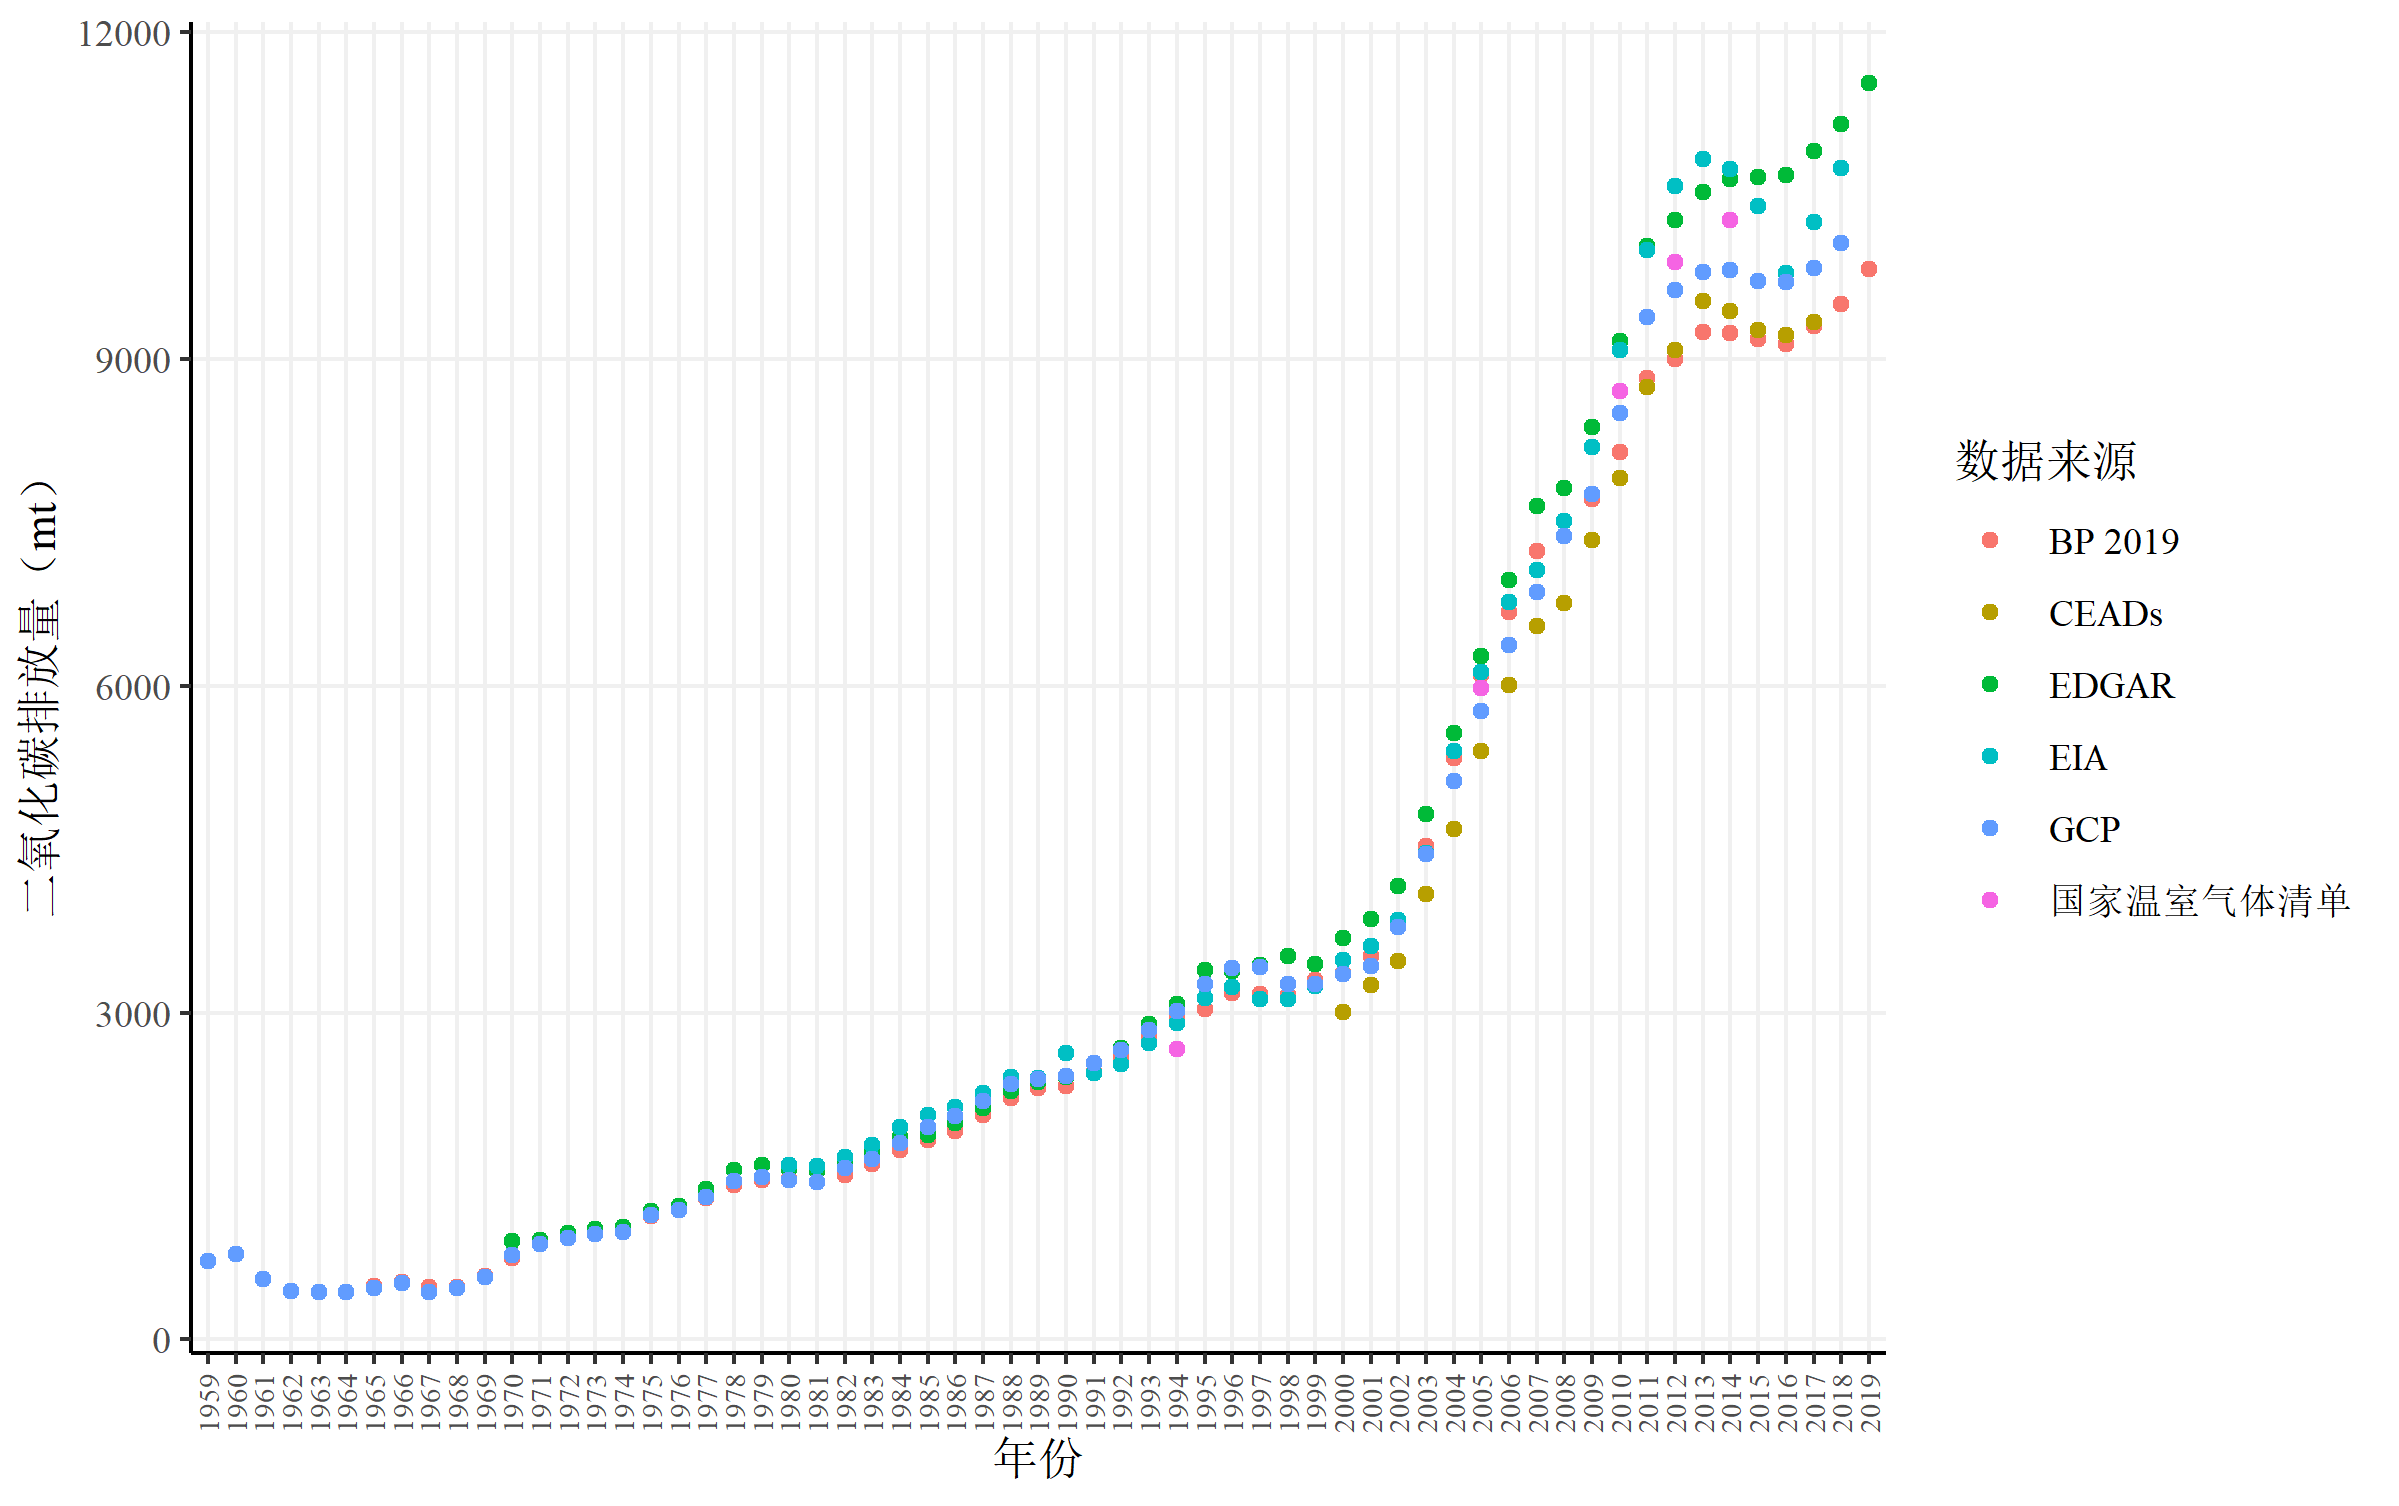
\includegraphics[width=5in]{emission.png}}
  \caption{中国1959-2019年二氧化碳排放量\label{fig:co2}}
  \vspace{1.5ex}
  \begin{minipage}{\textwidth}
    \small
    \phantom{缩进}注:如有需要可对图片进行注释说明,可省略。
    如有需要可对图片进行注释说明,可省略。
    如有需要可对图片进行注释说明,可省略。\\
    \phantom{缩进}图片来源:如需对图片来源进行说明,请参照此格式,可省略。
    如需对图片来源进行说明,请参照此格式,可省略。
  \end{minipage}
\end{figure}
\vspace{-3ex}
\zhlipsum

\subsection{三级标题}
\zhlipsum* 进一步阅读\cite{__2017,schmitt-grohe_covid-19_2020,__2020,__2019}。








% -*- coding:utf-8 -*-

\chapter{第二章}
\zhlipsum

\section{二级标题}
\zhlipsum

\subsection{三级标题}
\zhlipsum*[1]
\begin{equation}\label{eq:cdf}
  \operatorname{CDF}(x)=1-e^{-\theta x}
\end{equation}
根据公式(\ref{eq:cdf})和 $X=(I-A)^{-1}F$。
\zhlipsum
% -*- coding:utf-8 -*-

\chapter{一级标题}
正文正文正文正文正文正文正文正文正文正文正文正文。文正文正文正文正文正文。
正文正文正文正文正文正文正文正文正文正文正文正文正文正文正文正文正文正文。
正文正文正文正文正文正文正文正文正文正文正文正文正文正文正文正文正文正文。
正文正文正文正文正文正文正文正文正文正文正文正文正文正文正文正文正文正文。
正文正文正文正文正文正文正文正文正文正文正文正文正文正文正文正文正文正文。
正文正文正文正文正文正文正文正文正文正文正文正文正文正文正文正文正文正文。
正文正文正文正文正文正文正文正文正文正文正文正文正文正文正文正文正文正文。
正文正文正文正文正文正文正文正文正文正文正文正文正文正文正文正文正文正文。
正文正文正文正文正文正文正文正文正文正文正文正文正文正文正文正文正文正文。

\section{二级标题}
正文正文正文正文正文\footnote{\url{https://data.stats.gov.cn}}。正文。
正文正文正文正文正文正文正文正文正文正文正文正文正文正文正文正文正文正文。
正文正文正文正文正文正文正文正文正文正文正文正文正文正文正文正文正文正文。
正文正文正文正文正文正文正文正文正文正文正文正文正文正文正文正文正文正文。
正文正文正文正文正文正文正文正文正文正文正文正文正文正文正文正文正文正文。
正文正文正文正文正文正文正文正文正文正文正文正文正文正文正文正文正文正文。
正文正文正文正文正文正文正文正文正文正文正文正文正文正文正文正文正文正文。
正文正文正文正文正文正文正文正文正文正文正文正文正文正文正文正文正文正文。
正文正文正文正文正文正文正文正文正文正文正文正文正文正文正文正文正文正文。
正文正文正文正文正文正文正文正文正文正文正文正文正文正文正文正文正文正文。
正文正文正文正文正文正文正文正文正文正文正文正文正文正文正文正文正文正文。

表\ref{tab:example1}正文正文正文正文正文正文正文正文正文正文正文正文。
正文正文正文正文正文正文正文正文正文正文正文正文正文正文正文正文正文正文。
正文正文正文正文正文正文正文正文正文正文正文正文正文正文正文正文正文正文。
正文正文正文正文正文正文正文正文正文正文正文正文正文正文正文正文正文正文。
正文正文正文正文正文正文正文正文正文正文正文正文正文正文正文正文正文正文。
正文正文正文正文正文正文正文正文正文正文正文正文正文正文正文正文正文正文。
正文正文正文正文正文正文正文正文正文正文正文正文正文正文正文正文正文正文。
正文正文正文正文正文正文正文正文正文正文正文正文正文正文正文正文正文正文。
正文正文正文正文正文正文正文正文正文正文正文正文正文正文正文正文正文正文。

\begin{table}[H]
  \small
  \caption{表格标题表格标题表格标题\label{tab:example1}}
  \adjustbox{center}{%
    \begin{tabular}{lrrrrrrrr}
    \toprule  
  & \multicolumn{1}{l}{内容} & \multicolumn{1}{l}{内容} & \multicolumn{1}{l}{内容} & \multicolumn{1}{l}{内容} & \multicolumn{1}{l}{内容} & \multicolumn{1}{l}{内容} & \multicolumn{1}{l}{内容} & \multicolumn{1}{l}{内容} \\
    \midrule
    表格内容  & 123   & 4.56 & 7.89 & 5.67 & 7.89 & 1.23 & -4.56 & 7.89 \\
    表格内容  & 123   & 4.56 & 7.89 & 5.67 & 7.89  & 10.23 & 2.38 & 11.64 \\
    \bottomrule
  \end{tabular}}%
  \vspace{1.5ex}
  \begin{minipage}{\textwidth}
    \phantom{缩进}注:如有需要可对表格进行注释说明,可省略。
    如有需要可对表格进行注释说明,可省略。
    如有需要可对表格进行注释说明,可省略。\\
    \phantom{缩进}数据来源:如需对数据来源进行说明,请参照此格式,可省略。 
    如需对数据来源进行说明,请参照此格式,可省略。
  \end{minipage}
\end{table}%
\vspace{-3ex}
正文正文正文正文正文正文正文正文正文正文正文正文正文正文正文正文正文正文。
正文正文正文正文正文正文正文正文正文正文正文正文正文正文正文正文正文正文。
正文正文正文正文正文正文正文正文正文正文正文正文正文正文正文正文正文正文。
正文正文正文正文正文正文正文正文正文正文正文正文正文正文正文正文正文正文。
正文正文正文正文正文正文正文正文正文正文正文正文正文正文正文正文正文正文。
正文正文正文正文正文正文正文正文正文正文正文正文正文正文正文正文正文正文。
正文正文正文正文正文正文正文正文正文正文正文正文正文正文正文正文正文正文。
正文正文正文正文正文正文正文正文正文正文正文正文正文正文正文正文正文正文。
正文正文正文正文正文正文正文正文正文正文正文正文正文正文正文正文正文正文。

\subsection{三级标题}
正文正文正文正文正文正文正文正文正文正文正文正文正文正文正文正文正文正文。
正文正文正文正文正文正文正文正文正文正文正文正文正文正文正文正文正文正文。
正文正文正文正文正文正文正文正文正文正文正文正文正文正文正文正文正文正文。
正文正文正文正文正文正文正文正文正文正文正文正文正文正文正文正文正文正文。
正文正文正文正文正文正文正文正文正文正文正文正文正文正文正文正文正文正文。
正文正文正文正文正文正文正文正文正文正文正文正文正文正文正文正文正文正文。
正文正文正文正文正文正文正文正文正文正文正文正文正文正文正文正文正文正文。
正文正文正文正文正文正文正文正文正文正文正文正文正文正文正文正文正文正文。
正文正文正文正文正文正文正文正文正文正文正文正文图\ref{fig:CO_2}。

\begin{figure}[H]
  \adjustbox{center}{%
  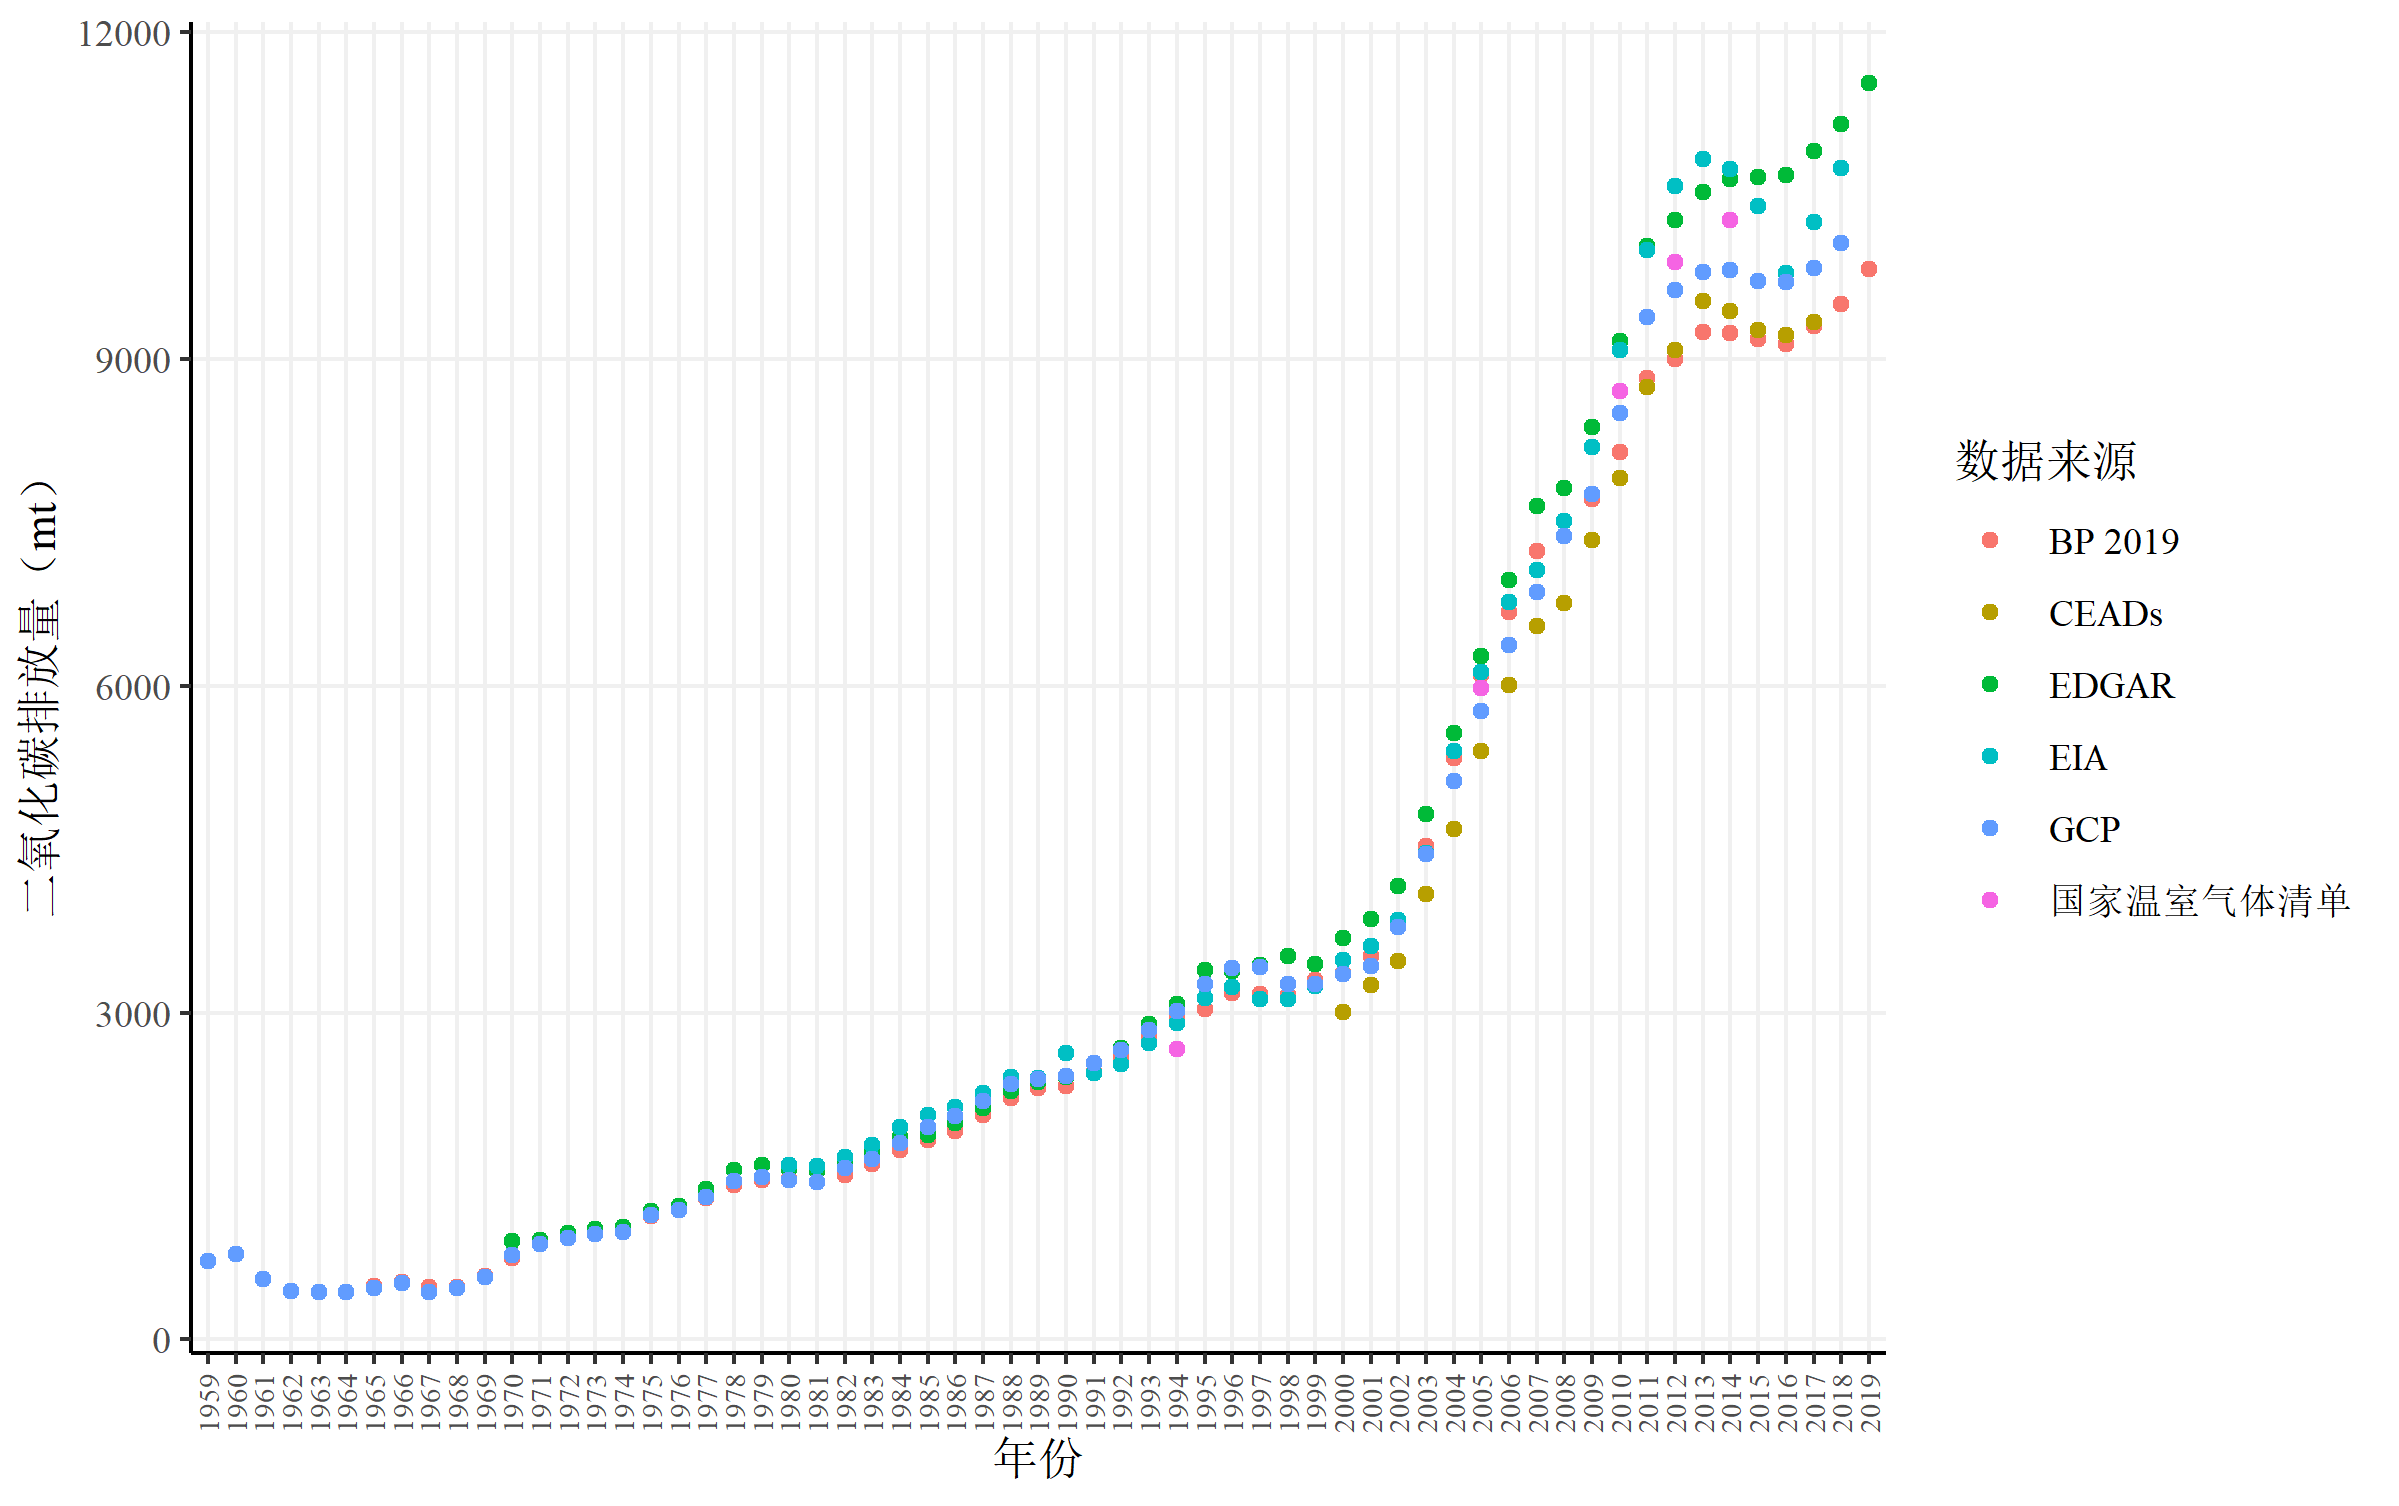
\includegraphics[width=5in]{emission.png}}
  \caption{中国1959-2019年二氧化碳排放量\label{fig:CO_2}}
\end{figure}

正文正文正文正文正文正文正文正文正文正文正文正文正文正文正文正文正文正文。
正文正文正文正文正文正文正文正文正文正文正文正文正文正文正文正文正文正文。
正文正文正文正文正文正文正文正文正文正文正文正文正文正文正文正文正文正文。
正文正文正文正文正文正文正文正文正文正文正文正文正文正文正文正文正文正文。
正文正文正文正文正文正文正文正文正文正文正文正文正文正文正文正文正文正文。
正文正文正文正文正文正文正文正文正文正文正文正文正文图\ref{fig:side_1}。

\hvFloat[%
capPos=bottom,
rotAngle=-90,
objectPos=center]%
{figure}{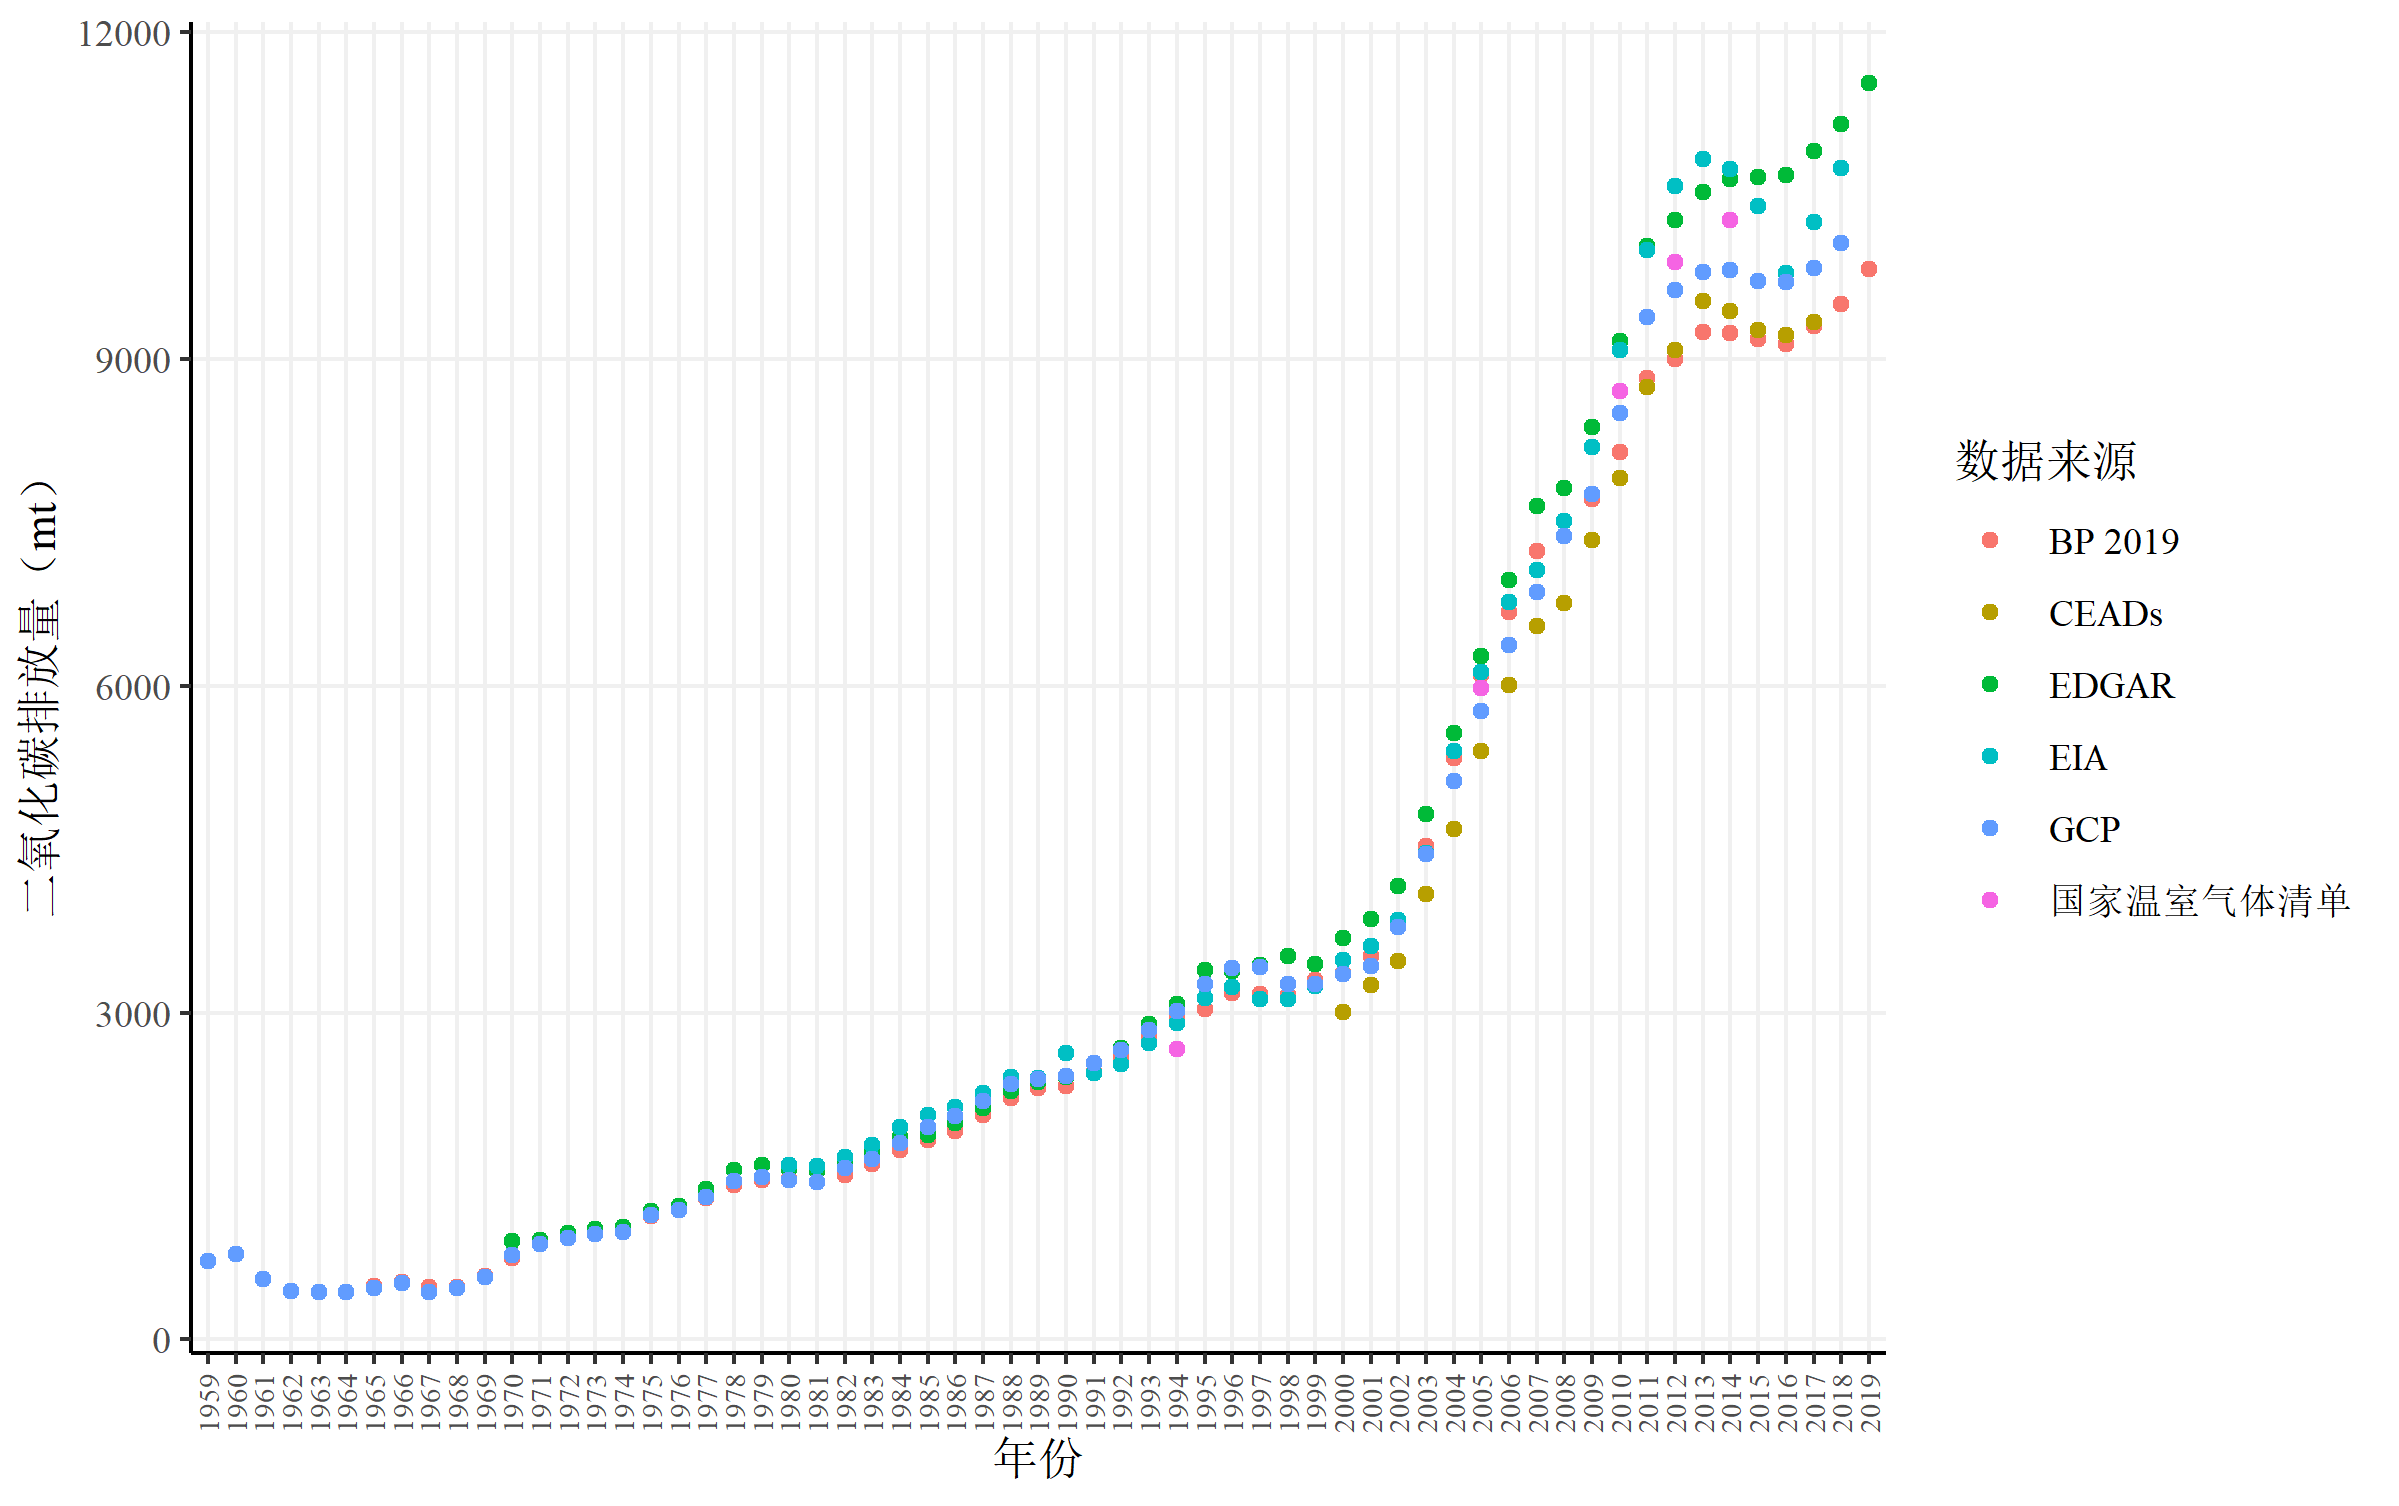
\includegraphics[width=5in]{emission.png}}
{中国1959-2019年二氧化碳排放量}{fig:side_1}
\vspace{-5ex}
正文正文正文正文正文正文正文正文正文正文正文正文正文正文正文正文正文正文。
正文正文正文正文正文正文正文正文正文正文正文正文正文正文正文正文正文正文。
正文正文正文正文正文正文正文正文正文正文正文正文正文正文正文正文正文正文。
正文正文正文正文正文正文正文正文正文正文正文正文正文正文正文正文正文正文。
正文正文正文正文正文正文正文正文正文正文正文正文正文正文正文正文正文正文。
正文正文正文正文正文正文正文正文正文正文正文正文正文正文正文正文正文正文。
正文正文正文正文正文正文正文正文正文正文正文正文正文正文正文正文正文正文。
正文正文正文正文正文正文正文正文正文正文正文正文正文正文正文正文正文正文。
正文正文正文正文正文正文正文图\ref{fig:side_2}正文正文正文正文正文。

\hvFloat[%
capPos=bottom,
rotAngle=90,
objectPos=center]%
{figure}{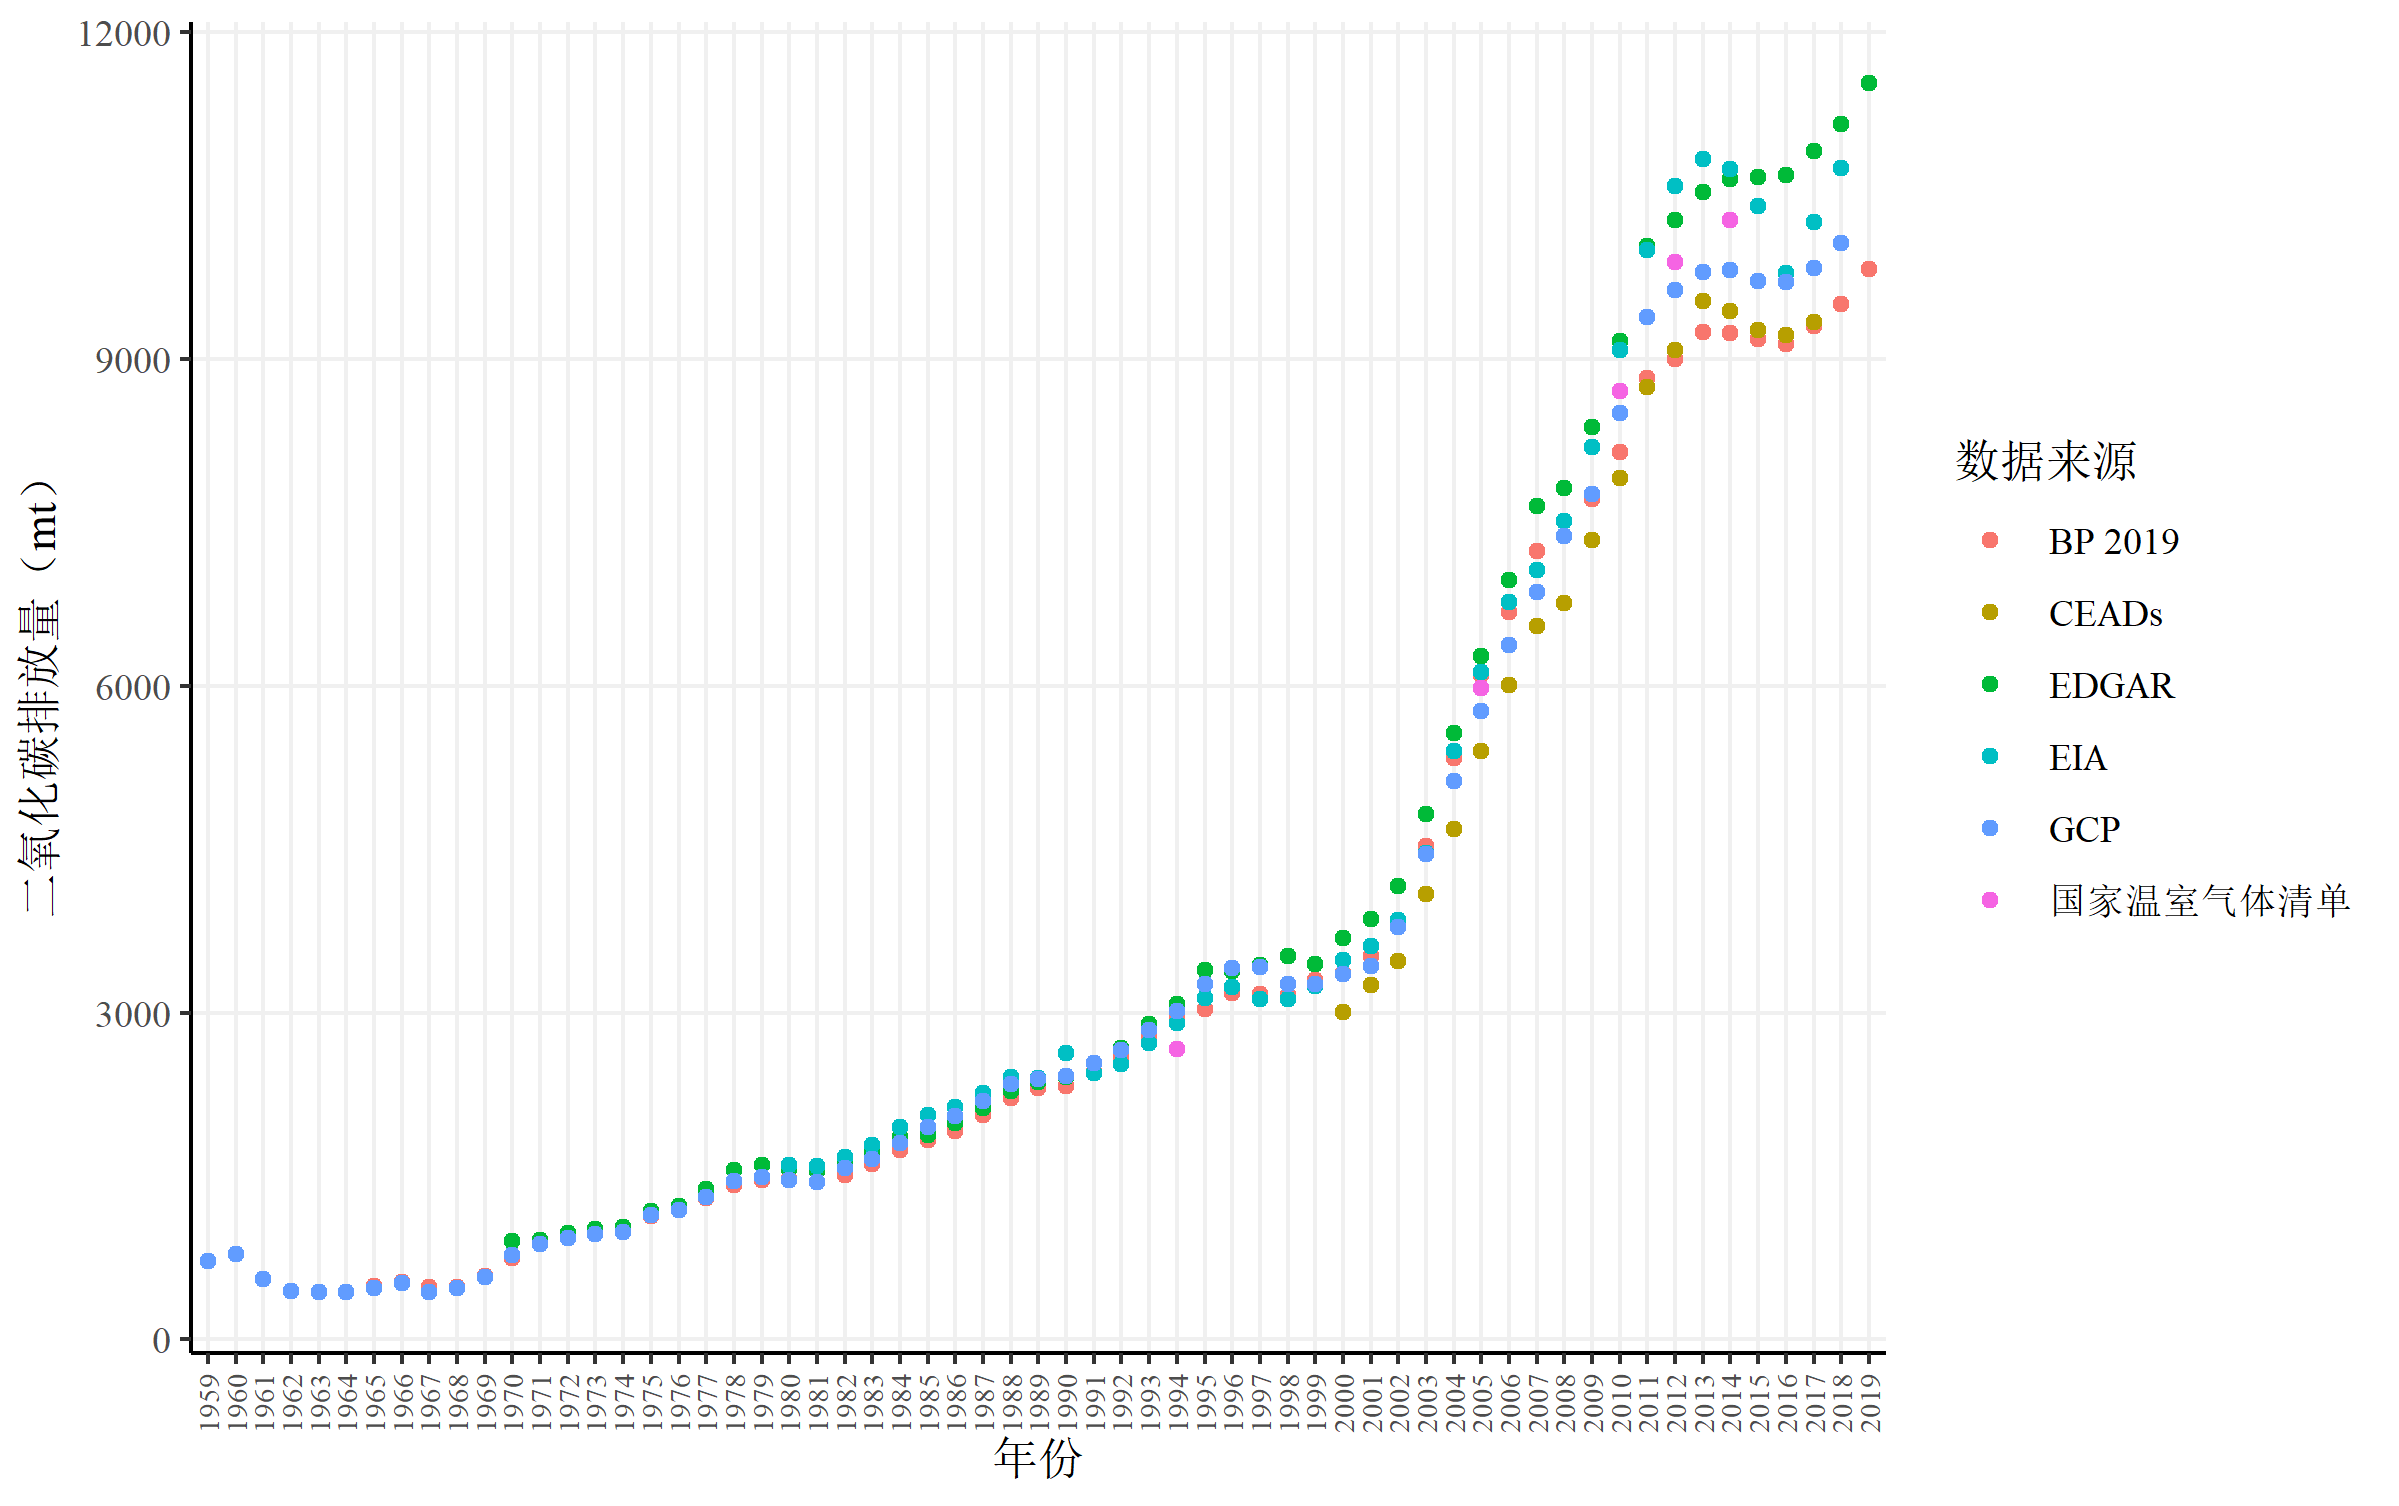
\includegraphics[width=5in]{emission.png}}
{中国1959-2019年二氧化碳排放量}{fig:side_2}
\vspace{-5ex}
正文正文正文正文正文正文正文正文正文正文正文正文正文正文正文正文正文正文。
正文正文正文正文正文正文正文正文正文正文正文正文正文正文正文正文正文正文。
正文正文正文正文正文正文正文正文正文正文正文正文正文正文正文正文正文正文。
正文正文正文正文正文正文正文正文正文正文正文正文正文正文正文正文正文正文。
正文正文正文正文正文正文正文正文正文正文正文正文正文正文正文正文正文正文。
正文正文正文正文(见表\ref{tab:side_1}和表\ref{tab:side_2})。

\savebox{\hvOBox}{%
\small
%\renewcommand{\arraystretch}{0.8} % 如果横置还是超宽,可以适当缩小表格行间距
\begin{tabular}{llrrrrrrrrrrrr}
  \toprule
  \multirow{2}[4]{*}{变量} & \multirow{2}[4]{*}{变量变量} & \multicolumn{1}{c}{\multirow{2}[4]{*}{变量}} & \multicolumn{5}{c}{变量}             & \multicolumn{5}{c}{变量}             & \multicolumn{1}{c}{\multirow{2}[4]{*}{变量}} \\
\cmidrule{4-13}          &       &       & \multicolumn{1}{c}{0} & \multicolumn{1}{c}{1} & \multicolumn{1}{c}{2} & \multicolumn{1}{c}{3} & \multicolumn{1}{c}{4} & \multicolumn{1}{c}{0} & \multicolumn{1}{c}{1} & \multicolumn{1}{c}{2} & \multicolumn{1}{c}{3} & \multicolumn{1}{c}{4} &  \\
  \midrule
  \multirow{6}[2]{*}{正文正文} & 正文正文  & 0.01  & 0.01  & 0.01  & 0.01  & 0.01  & 0.01  & 0.01  & 0.01  & 0.01  & 0.01  & 0.01  & \multicolumn{1}{c}{0.01} \\
        & 正文正   & 0.01  & 0.01 & 0.01  & 0.01  & 0.01  & 0.01 & 0.01  & 0.01  & 0.01  & 0.01  & 0.01  & \multicolumn{1}{c}{0.01} \\
        & 正文正文  & 0.01  & 0.01  & 0.01  & 0.01  & 0.01  & 0.01  & 0.01  & 0.01  & 0.01  & 0.01  & 0.01  & \multicolumn{1}{c}{0.01} \\
        & 正文正正文 & 0.01  & 0.01  & 0.01  & 0.01  & 0.01  & 0.01  & 0.01  & 0.01  & 0.01  & 0.01  & 0.01  & \multicolumn{1}{c}{0.01} \\
        & 正文正文正文正文正文正文正文 & 0.01  & 0.01  & 0.01  & 0.01  & 0.01  & 0.01  & 0.01  & 0.01  & 0.01  & 0.01  & 0.01  & \multicolumn{1}{c}{0.01} \\
        & 正文、正文正正文 & 0.01  & 0.01  & 0.01  & 0.01  & 0.01  & 0.01  & 0.01  & 0.01  & 0.01  & 0.01  & 0.01  & \multicolumn{1}{c}{0.01} \\
\cmidrule{1-2}    \multirow{6}[2]{*}{正文正文} & 正文正正文 & 0.01  & 0.01  & 0.01  & 0.01  & 0.01  & 0.01  & 0.01  & 0.01  & 0.01  & 0.01  & 0.01  & \multicolumn{1}{c}{0.01} \\
        & 正文正正文正文正文 & 0.01  & 0.01  & 0.01  & 10.01  & 11.01  & 0.01  & 0.01  & 10.01  & 10.01  & 10.01  & 10.01  & \multicolumn{1}{c}{0.01} \\
        & 正文正正文正文正正文 & 10.01  & 10.01  & 0.01  & 10.01  & 10.01  & 0.01  & 10.01  & 10.01  & 10.01  & 10.01  & 10.01  & \multicolumn{1}{c}{0.01} \\
        & 正文正文正文正正文 & 0.01  & 0.01  & 0.01  & 0.01  & 10.01  & 0.01  & 0.01  & 0.01  & 0.01  & 0.01  & 0.01  & \multicolumn{1}{c}{1.18 } \\
        & 正文正文正文正文正文正文正文正 & 0.01  & 0.01  & 0.01  & 0.01  & 0.01  & 0.01  & 0.01  & 0.01  & 0.01  & 0.01  & 0.01  & \multicolumn{1}{c}{0.01} \\
        & 正文正文正文正文正文正文正文 & 0.01  & 0.01  & 0.01  & 0.01  & 0.01  & 0.01  & 0.01  & 0.01  & 0.01  & 0.01  & 0.01  & 0.01  \\
  \bottomrule
\end{tabular}%
}
\hvFloat[%
floatPos=hb,
useOBox=true,
objectAngle=-90,
capAngle=-90,
capPos=right,
capWidth=w]%
{table}{}{超宽表格横置示例}{tab:side_1}

\savebox{\hvOBox}{%
\small
%\renewcommand{\arraystretch}{0.8} % 如果横置还是超宽,可以适当缩小表格行间距
\begin{tabular}{llrrrrrrrrrrrr}
  \toprule
  \multirow{2}[4]{*}{变量} & \multirow{2}[4]{*}{变量变量} & \multicolumn{1}{c}{\multirow{2}[4]{*}{变量}} & \multicolumn{5}{c}{变量}             & \multicolumn{5}{c}{变量}             & \multicolumn{1}{c}{\multirow{2}[4]{*}{变量}} \\
\cmidrule{4-13}          &       &       & \multicolumn{1}{c}{0} & \multicolumn{1}{c}{1} & \multicolumn{1}{c}{2} & \multicolumn{1}{c}{3} & \multicolumn{1}{c}{4} & \multicolumn{1}{c}{0} & \multicolumn{1}{c}{1} & \multicolumn{1}{c}{2} & \multicolumn{1}{c}{3} & \multicolumn{1}{c}{4} &  \\
  \midrule
  \multirow{6}[2]{*}{正文正文} & 正文正文  & 0.01  & 0.01  & 0.01  & 0.01  & 0.01  & 0.01  & 0.01  & 0.01  & 0.01  & 0.01  & 0.01  & \multicolumn{1}{c}{0.01} \\
        & 正文正   & 0.01  & 0.01 & 0.01  & 0.01  & 0.01  & 0.01 & 0.01  & 0.01  & 0.01  & 0.01  & 0.01  & \multicolumn{1}{c}{0.01} \\
        & 正文正文  & 0.01  & 0.01  & 0.01  & 0.01  & 0.01  & 0.01  & 0.01  & 0.01  & 0.01  & 0.01  & 0.01  & \multicolumn{1}{c}{0.01} \\
        & 正文正正文 & 0.01  & 0.01  & 0.01  & 0.01  & 0.01  & 0.01  & 0.01  & 0.01  & 0.01  & 0.01  & 0.01  & \multicolumn{1}{c}{0.01} \\
        & 正文正文正文正文正文正文正文 & 0.01  & 0.01  & 0.01  & 0.01  & 0.01  & 0.01  & 0.01  & 0.01  & 0.01  & 0.01  & 0.01  & \multicolumn{1}{c}{0.01} \\
        & 正文、正文正正文 & 0.01  & 0.01  & 0.01  & 0.01  & 0.01  & 0.01  & 0.01  & 0.01  & 0.01  & 0.01  & 0.01  & \multicolumn{1}{c}{0.01} \\
\cmidrule{1-2}    \multirow{6}[2]{*}{正文正文} & 正文正正文 & 0.01  & 0.01  & 0.01  & 0.01  & 0.01  & 0.01  & 0.01  & 0.01  & 0.01  & 0.01  & 0.01  & \multicolumn{1}{c}{0.01} \\
        & 正文正正文正文正文 & 0.01  & 0.01  & 0.01  & 10.01  & 11.01  & 0.01  & 0.01  & 10.01  & 10.01  & 10.01  & 10.01  & \multicolumn{1}{c}{0.01} \\
        & 正文正正文正文正正文 & 10.01  & 10.01  & 0.01  & 10.01  & 10.01  & 0.01  & 10.01  & 10.01  & 10.01  & 10.01  & 10.01  & \multicolumn{1}{c}{0.01} \\
        & 正文正文正文正正文 & 0.01  & 0.01  & 0.01  & 0.01  & 10.01  & 0.01  & 0.01  & 0.01  & 0.01  & 0.01  & 0.01  & \multicolumn{1}{c}{1.18 } \\
        & 正文正文正文正文正文正文正文正 & 0.01  & 0.01  & 0.01  & 0.01  & 0.01  & 0.01  & 0.01  & 0.01  & 0.01  & 0.01  & 0.01  & \multicolumn{1}{c}{0.01} \\
        & 正文正文正文正文正文正文正文 & 0.01  & 0.01  & 0.01  & 0.01  & 0.01  & 0.01  & 0.01  & 0.01  & 0.01  & 0.01  & 0.01  & 0.01  \\
  \bottomrule
\end{tabular}%
}
\hvFloat[%
floatPos=hb,
useOBox=true,
objectAngle=90,
capAngle=90,
capPos=left,
capWidth=w]%
{table}{}{超宽表格横置示例}{tab:side_2}










\renewcommand*{\bibfont}{\small}
\printbibliography[heading=bibintoc]                  % 插入参考文献 biblatex

\chapter*{致谢}
\addcontentsline{toc}{chapter}{致谢}
致谢致谢致谢致谢致谢致谢致谢致谢致谢致谢致谢致谢。
致谢致谢致谢致谢致谢致谢致谢致谢致谢致谢致谢致谢。
致谢致谢致谢致谢致谢致谢致谢致谢致谢致谢致谢致谢。
致谢致谢致谢致谢致谢致谢致谢致谢致谢致谢致谢致谢。
致谢致谢致谢致谢致谢致谢致谢致谢致谢致谢致谢致谢。

致谢致谢致谢致谢致谢致谢致谢致谢致谢致谢致谢致谢。
致谢致谢致谢致谢致谢致谢致谢致谢致谢致谢致谢致谢。
致谢致谢致谢致谢致谢致谢致谢致谢致谢致谢致谢致谢。
致谢致谢致谢致谢致谢致谢致谢致谢致谢致谢致谢致谢。
致谢致谢致谢致谢致谢致谢致谢致谢致谢致谢致谢致谢。

\appendix					    % 开始附录
% -*- coding:utf-8 -*-

\chapter{长表格示例}

% Please add the following required packages to your document preamble:
% \usepackage{booktabs}
\begin{small}
    \begin{longtabu} to \textwidth {X[-1cp]X[1cp]}
        \caption{产业部门划分表}\\
        \toprule
        序号&
        2018年投入产出表产业部门名称\\
        \midrule
        \endfirsthead

        \multicolumn{2}{c}{(续表)}\\
        \toprule
        序号&
        2018年投入产出表产业部门名称\\
        \midrule
        \endhead

        \bottomrule
        \multicolumn{2}{c}{接下一页表格……}\\
        \endfoot

        \bottomrule
        \endlastfoot

        1   & 农产品                \\
        2   & 林产品                \\
        3   & 畜牧产品               \\
        4   & 渔产品                \\
        5   & 农、林、牧、渔服务产品        \\
        6   & 煤炭开采和洗选产品          \\
        7   & 石油和天然气开采产品         \\
        8   & 黑色金属矿采选产品          \\
        9   & 有色金属矿采选产品          \\
        10  & 非金属矿采选产品           \\
        11  & 开采辅助活动和其他采矿产品      \\
        12  & 谷物磨制品              \\
        13  & 饲料加工品              \\
        14  & 植物油加工品             \\
        15  & 糖及糖制品              \\
        16  & 屠宰及肉类加工品           \\
        17  & 水产加工品              \\
        18  & 蔬菜、水果、坚果和其他农副食品加工品 \\
        19  & 方便食品               \\
        20  & 乳制品                \\
        21  & 调味品、发酵制品           \\
        22  & 其他食品               \\
        23  & 酒精和酒               \\
        24  & 饮料                 \\
        25  & 精制茶                \\
        26  & 烟草制品               \\
        27  & 棉、化纤纺织及印染精加工品      \\
        28  & 毛纺织及染整精加工品         \\
        29  & 麻、丝绢纺织及加工品         \\
        30  & 针织或钩针编织及其制品        \\
        31  & 纺织制成品              \\
        32  & 纺织服装服饰             \\
        33  & 皮革、毛皮、羽毛及其制品       \\
        34  & 鞋                  \\
        35  & 木材加工和木、竹、藤、棕、草制品   \\
        36  & 家具                 \\
        37  & 造纸和纸制品             \\
        38  & 印刷和记录媒介复制品         \\
        39  & 工艺美术品              \\
        40  & 文教、体育和娱乐用品         \\
        41  & 精炼石油和核燃料加工品        \\
        42  & 煤炭加工品              \\
        43  & 基础化学原料             \\
        44  & 肥料                 \\
        45  & 农药                 \\
        46  & 涂料、油墨、颜料及类似产品      \\
        47  & 合成材料               \\
        48  & 专用化学产品和炸药、火工、焰火产品  \\
        49  & 日用化学产品             \\
        50  & 医药制品               \\
        51  & 化学纤维制品             \\
        52  & 橡胶制品               \\
        53  & 塑料制品               \\
        54  & 水泥、石灰和石膏           \\
        55  & 石膏、水泥制品及类似制品       \\
        56  & 砖瓦、石材等建筑材料         \\
        57  & 玻璃和玻璃制品            \\
        58  & 陶瓷制品               \\
        59  & 耐火材料制品             \\
        60  & 石墨及其他非金属矿物制品       \\
        61  & 钢                  \\
        62  & 钢压延产品              \\
        63  & 铁及铁合金产品            \\
        64  & 有色金属及其合金           \\
        65  & 有色金属压延加工品          \\
        66  & 金属制品               \\
        67  & 锅炉及原动设备            \\
        68  & 金属加工机械             \\
        69  & 物料搬运设备             \\
        70  & 泵、阀门、压缩机及类似机械      \\
        71  & 烘炉、风机、包装等设备        \\
        72  & 文化、办公用机械           \\
        73  & 其他通用设备             \\
        74  & 采矿、冶金、建筑专用设备       \\
        75  & 化工、木材、非金属加工专用设备    \\
        76  & 农、林、牧、渔专用机械        \\
        77  & 医疗仪器设备及器械          \\
        78  & 其他专用设备             \\
        79  & 汽车整车               \\
        80  & 汽车零部件及配件           \\
        81  & 铁路运输和城市轨道交通设备      \\
        82  & 船舶及相关装置            \\
        83  & 其他交通运输设备           \\
        84  & 电机                 \\
        85  & 输配电及控制设备           \\
        86  & 电线、电缆、光缆及电工器材      \\
        87  & 电池                 \\
        88  & 家用器具               \\
        89  & 其他电气机械和器材          \\
        90  & 计算机                \\
        91  & 通信设备               \\
        92  & 广播电视设备和雷达及配套设备     \\
        93  & 视听设备               \\
        94  & 电子元器件              \\
        95  & 其他电子设备             \\
        96  & 仪器仪表               \\
        97  & 其他制造产品             \\
        98  & 废弃资源和废旧材料回收加工品     \\
        99  & 金属制品、机械和设备修理服务     \\
        100 & 电力、热力生产和供应         \\
        101 & 燃气生产和供应            \\
        102 & 水的生产和供应            \\
        103 & 住宅房屋建筑             \\
        104 & 体育场馆和其他房屋建筑        \\
        105 & 铁路、道路、隧道和桥梁工程建筑    \\
        106 & 其他土木工程建筑           \\
        107 & 建筑安装               \\
        108 & 建筑装饰、装修和其他建筑服务     \\
        109 & 批发                 \\
        110 & 零售                 \\
        111 & 铁路旅客运输             \\
        112 & 铁路货物运输和运输辅助活动      \\
        113 & 城市公共交通及公路客运        \\
        114 & 道路货物运输和运输辅助活动      \\
        115 & 水上旅客运输             \\
        116 & 水上货物运输和运输辅助活动      \\
        117 & 航空旅客运输             \\
        118 & 航空货物运输和运输辅助活动      \\
        119 & 管道运输               \\
        120 & 多式联运和运输代理          \\
        121 & 装卸搬运和仓储            \\
        122 & 邮政                 \\
        123 & 住宿                 \\
        124 & 餐饮                 \\
        125 & 电信                 \\
        126 & 广播电视及卫星传输服务        \\
        127 & 互联网和相关服务           \\
        128 & 软件服务               \\
        129 & 信息技术服务             \\
        130 & 货币金融和其他金融服务        \\
        131 & 资本市场服务             \\
        132 & 保险                 \\
        133 & 房地产                \\
        134 & 租赁                 \\
        135 & 商务服务               \\
        136 & 研究和试验发展            \\
        137 & 专业技术服务             \\
        138 & 科技推广和应用服务          \\
        139 & 水利管理               \\
        140 & 生态保护和环境治理          \\
        141 & 公共设施及土地管理          \\
        142 & 居民服务               \\
        143 & 其他服务               \\
        144 & 教育                 \\
        145 & 卫生                 \\
        146 & 社会工作               \\
        147 & 新闻和出版              \\
        148 & 广播、电视、电影和影视录音制作    \\
        149 & 文化艺术               \\
        150 & 体育                 \\
        151 & 娱乐                 \\
        152 & 社会保障               \\
        153 & 公共管理和社会组织          \\
    \end{longtabu}
\end{small}		% 附录A
% -*- coding:utf-8 -*-

\chapter{简历}
\subsection*{个人简介}
杨过,男,汉族,中国人,武学学士,硕士研究生。

\subsection*{发表论文}
\begin{small}   
\noindent [1] \textbf{Yang G}, Guo J. A study on the origin of the Eighteen Dragon-Subduing Palms[J]. Journal of Martial Arts, 1248, 227: 263–271.

\noindent [2] \heiti{杨过}, \songti{郭靖}.\songti{打狗棒法的改进}[J]. \songti{武术研究}, 1249, 36(09): 158–165.
\end{small}
				% 简历
\end{document}